\section{Basics}


\subsection{Default Parameterization}

From the user's point of view, this package's simplest entry point is:

\ccFunction{Parameterizer_traits_3<ParameterizationMesh_3>::Error_code parameterize (ParameterizationMesh_3 * mesh);}
{
Compute a 1 to 1 mapping from a triangular 3D surface 'mesh' to 2D circle, using
Floater Mean Value Coordinates algorithm. 1 to 1 mapping is guaranteed.
The mapping is linear by pieces (linear in each triangle). The result is the (u,v) pair image of each vertex of the 3D surface.
Preconditions:\begin{itemize}
\item 'mesh' must be a surface with 1 connected component.\item 'mesh' must be a triangular mesh.\end{itemize}
}

This CGAL::parameterize() function provides a default parameterization method:
Floater Mean Value Coordinates \cite{cgal:f-mvc-03}, with an arc length circular border
parameterization, and using OpenNL sparse linear solver \cite{cgal:l-nmdgp-05}.

The result is stored in the (u,v) fields of the mesh's vertices and/or halfedges.

% Include floater.png/eps figure with title = "Floater Mean Value Coordinates parameterization"
\begin{figure}[bht]
    \begin{center}
        % Image
        \begin{ccTexOnly}
            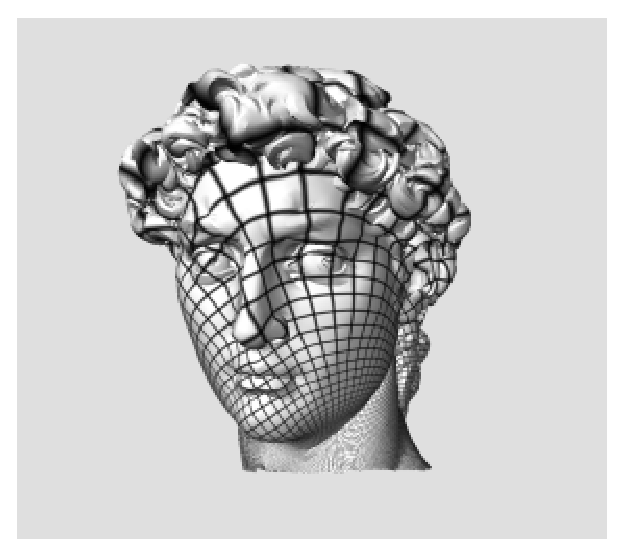
\includegraphics{Parameterization/floater} % omit suffix to support PS and PDF
        \end{ccTexOnly}
        \begin{ccHtmlOnly}
            <img border=0 src="./floater.png" align=center>
        \end{ccHtmlOnly}
        \label{parameterization-fig-floater}

        % Title
        \caption{Floater Mean Value Coordinates}
    \end{center}
\end{figure}


\subsection{Supported Meshes List and Concept}

The general definition of input meshes handled by the package is:

\begin{itemize}

\item Triangulated.

\item 2-manifold.

\item Oriented.

\item Surface parameterization methods deal only with topological discs.
The input mesh can be of any genus and have any number of connected components.
If it is not a topological disc, it has to come with a description of a border
(a list of vertices) which is the border of a topological disc.
If no border is given, we assume that the surface border
is the longest border already in the input mesh (the other borders will
be considered as holes).

Note that this way the user is responsible for cutting a closed mesh of
arbitrary genus (even a topological disc with an intricate seam
cut), as long as this condition is fulfilled.

The package will only parameterize the inside part of the given border,
thus only one connected component.

\end{itemize}

The package accesses such meshes through the \ccc{ParameterizationMesh_3} concept. Among other
things, this concept defines the accessor to the (u,v) values computed
by parameterizations.

The package offers models of the concept
\ccc{ParameterizationMesh_3} with both the 2D Triangulation Data Structure enriched
with 3D points (not yet implemented) and the Polyhedron:

\ccc{CGAL::Parameterization_polyhedron_adaptor_3}  \\

Note that these interfaces are decorators that add {\em on the fly} the necessary
fields to unmodified CGAL data structures (using STL maps).
For performance reasons, it is recommended to use CGAL data structures
enriched with the proper fields.
See \ccc{Polyhedron_ex} class in \ccc{polyhedron_ex_parameterization.C} example.


\subsection{Default Parameterization Example}

The code below applies the default parameterization to a \ccc{Polyhedron_3} mesh:

\begin{ccExampleCode}

// CGAL kernel
typedef CGAL::Cartesian<double>                         Kernel;

// Mesh true type and parameterization adaptors
typedef CGAL::Polyhedron_3<Kernel>                      Polyhedron;
typedef CGAL::Parameterization_polyhedron_adaptor_3<Polyhedron>         
                                                        Parameterization_polyhedron_adaptor;

// Defines the error codes
typedef CGAL::Parameterizer_traits_3<Parameterization_polyhedron_adaptor> 
                                                        Parameterizer;

int main(int argc,char * argv[])
{
    Polyhedron mesh;
    ...

    // The parameterization package needs an adaptor to handle Polyhedron_3 meshes
    Parameterization_polyhedron_adaptor mesh_adaptor(&mesh);

    // Floater Mean Value Coordinates parameterization
    Parameterizer::Error_code err = CGAL::parameterize(&mesh_adaptor);
    ...
}

\end{ccExampleCode}

See the complete code in \ccc{Simple_parameterization.C} example.


